\section{Die Benutzerschnittstelle}
	In diesem Abschnitt dieses Kapitels wird auf die Implementierung der Benutzerschnittstelle eingegangen. Wie schon bereits im SRS erwähnt handelt es sich bei der Benutzerschnittstelle um die grafische Oberfläche der Android App. Dafür werden zunächst die Möglichkeiten von Unity vorgestellt, dann auf das Ergebnis der Umsetzung eingegangen und abschließend die Auswertung des Usability Tests behandelt.
	
	\subsection{Grafische Oberfläche mit Unity}
		Die grafische Oberfläche wird mit Unity's zur Verfügung gestelltem UI System implementiert. Der Canvas, zu deutsch Leinwand, stellt dabei die Hauptkomponente bzw. Elternkomponente dar. Alle UI Elemente sind Kinder des Canvas und erben somit die Eigenschaften des Canvas. Unity bietet standardmäßig eine große Anzahl an UI Elementen, wie beispielsweise Buttons, Toggle-Buttons, Dropdown-Listen und Eingabefelder\footnote{Vgl. \url{https://docs.unity3d.com/Manual/UIInteractionComponents.html}}. Der Canvas verwendet das EventSystem Objekt von Unity. Das Event System ermöglicht es, alle Touchscreen-Eingaben an die korrekten UI Elemente in der App weiterzuleiten\footnote{Vgl. \url{https://docs.unity3d.com/Manual/EventSystem.html}}.
		
		Bei der Implementierung des Canvas wird zwischen drei unterschiedlichen Render-Modi unterschieden\footnote{Vgl. \url{https://docs.unity3d.com/Manual/UICanvas.html}}. Je nachdem welcher Modus verwendet wird, ist die grafische Oberfläche anders in das Spiel integriert.
		
		\subsubsection{Screen Space - Overlay}
			Standardmäßig ist jedes Canvas als Screen Space - Overlay implementiert. Dieser Modus platziert die UI Elemente auf den Bildschirm über die komplette Szene. Die Benutzeroberfläche wird über alle anderen Grafiken, wie die Kamera-Ansicht, gezogen. Wenn die Auflösung geändert wird, passt der Canvas die Größe aller Kindelemente automatisch an die neue Auflösung an. Deshalb ist es besonders wichtig, dass alle UI Elemente unter dem Canvas hängen. 
			
			Die folgende Grafik\footnote{Bild entnommen von \url{https://docs.unity3d.com/Manual/class-Canvas.html}} \ref{renderOverlay} verdeutlicht, dass alle Elemente des Spieles hinter der Benutzeroberfläche positioniert sind.
			
			\begin{figure}[htbp]
				\centering 
				\label{renderOverlay}
				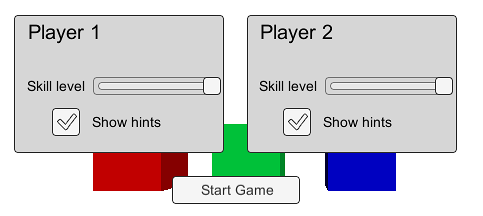
\includegraphics[width=10cm]{pics/CanvasOverlay.png}
				\caption{Render-Modus: Screen Space - Overlay}
			\end{figure}
			
			Die wesentliche Nachteile vom Screen Space - Overlay ist, dass der sichtbare Bereich des Spieles durch die UI Elemente verdeckt wird. Deshalb ist es besonders wichtig nur die wichtigsten Elementen immer sichtbar im Vordergrund zu lassen. Dies hat Auswirkungen auf die Positionen, Größe, Farbe und Design. Ein weiterer Nachteil ist, dass Spielelemente nicht als Teil des User Interfaces verwendet werden können. 
			
			Auf der Gegenseite können keine UI Elemente oder wichtige Informationen von den Gegenständen im Spiel verdeckt werden und ein weiterer Vorteil ist, dass die Position auf dem Bildschirm immer an die Auflösung angepasst wird und sich nicht ändert, unabhängig davon welche Aktionen der Spieler im Spiel ausführt oder auf welcher Hardware NoRPG gespielt wird.

		\subsubsection{Screen Space - Camera}
			Dieser Modus ähnelt dem ersten Modus sehr, aber in diesem Render-Modus wird der Canvas eine vorgegebene Distanz vor einer bestimmten Kamera platziert. Die UI Elemente werden von der bestimmen Kamera gerendert, was bedeutet, dass die Kameraeinstellungen das Erscheinungsbild der Benutzeroberfläche beeinflussen. Wenn sich die Auflösung des Bildschirms verkleinert, oder die Kameraposition und -winkel sich ändern, ändert sich der Canvas automatisch mit und passt die Größe der Elemente an.
			
			Der größte Unterschied ist allerdings, wenn 3D-Objekte in der Szene näher an der Kamera sind als die UI Elemente, werden diese auch auf dem Bildschirm vor der Benutzeroberfläche platziert. Dieses Verhalten wird in der folgenden Grafik\footnote{Bild entnommen von \url{https://docs.unity3d.com/Manual/class-Canvas.html}} \ref{renderCamera} deutlich.
			
			\begin{figure}[htbp]
				\centering 
				\label{renderCamera}
				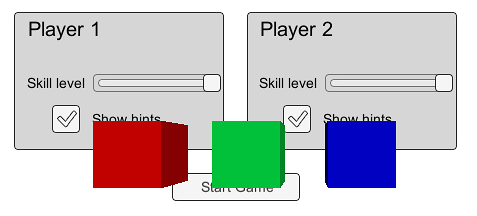
\includegraphics[width=10cm]{pics/CanvasCamera.png}
				\caption{Render-Modus: Screen Space - Camera}
			\end{figure}
		
			Wenn die 3D-Objekte näher als die UI-Elemente sind können Informationen und Elemente, wie Buttons, verdeckt werden und die Interaktion mit diesen Elementen ist nicht mehr möglich. Allerdings ermöglicht dieser Modus, dass Spielelemente als Teil der UI, auch wenn nur kurzfristig, funktionieren können. Trotz diesen Vorteils ist dieses Verhalten komplexer und fehleranfälliger.
		
		\subsubsection{World Space}
			In diesem Render-Modus wird der Canvas wie jedes andere Objekt in der Szene behandelt. Die Größe und Position kann manuell gesetzt werden und die UI Elemente werden basierend auf die 3D-Position entweder vor und hinter 3D-Objekten der Szene platziert. Dies ist nützlich für UIs, die dazu bestimmt sind, ein Teil der Welt zu sein. Dies wird auch als \"sterbliche\" Benutzeroberfläche bezeichnet, da diese nicht immer im Vordergrund sein muss. Im Gegensatz zum Screen Space - Camera Modus muss die UI Ebene nicht vor die Kamera platziert werden.
			
			Die Größe des Canvas kann manuell eingestellt werden, aber seine Größe auf dem Bildschirm wird von dem Winkel und der Entfernung der Kamera abhängen. Andere Szeneobjekte können hinter, mittendrin oder vor dem Canvas sein. Dieses Verhalten wird in folgender Grafik \footnote{Bild entnommen von \url{https://docs.unity3d.com/Manual/class-Canvas.html}} \ref{renderWorldSpace} deutlich.
			
			\begin{figure}[htbp]
				\centering 
				\label{renderWorldSpace}
				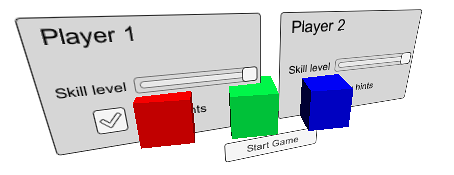
\includegraphics[width=10cm]{pics/CanvasWorldSpace.png}
				\caption{Render-Modus: World Space}
			\end{figure}
		
			Vor und Nachteile noch
			
	\subsection{Die Umsetzung}	
		Um die ergonomie zu erhöhen kann der linke joystick i einem festgelegten bereich überall angelegt werden
		
		Da es sich um KOmponenten handelt die immer da sein müssen wurde sich für das normale UI Screen Space - OVerlay ausgewählt
		
		\begin{figure}[htbp]
			\centering 
			\label{alwaysOnUI}
			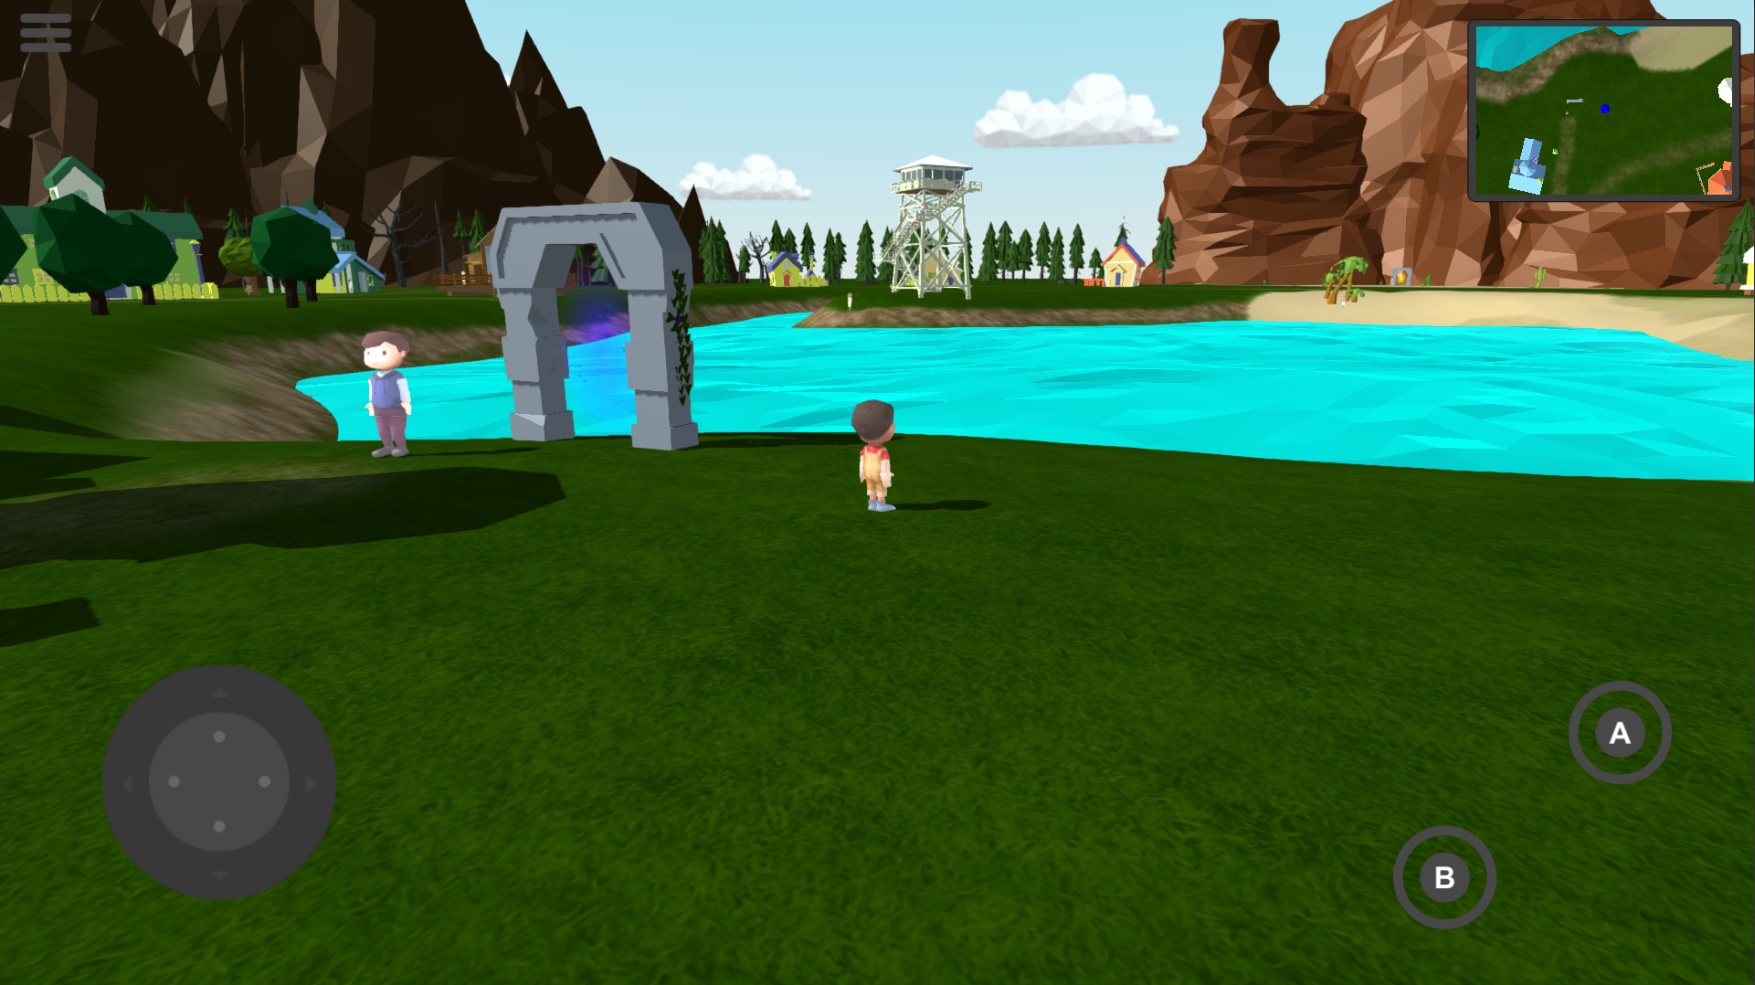
\includegraphics[width=13cm]{pics/alwaysOnUI.png}
			\caption{User Interface: Head-Up Display}
		\end{figure}
	
		\begin{figure}[htbp]
			\centering 
			\label{userInterfaces}
			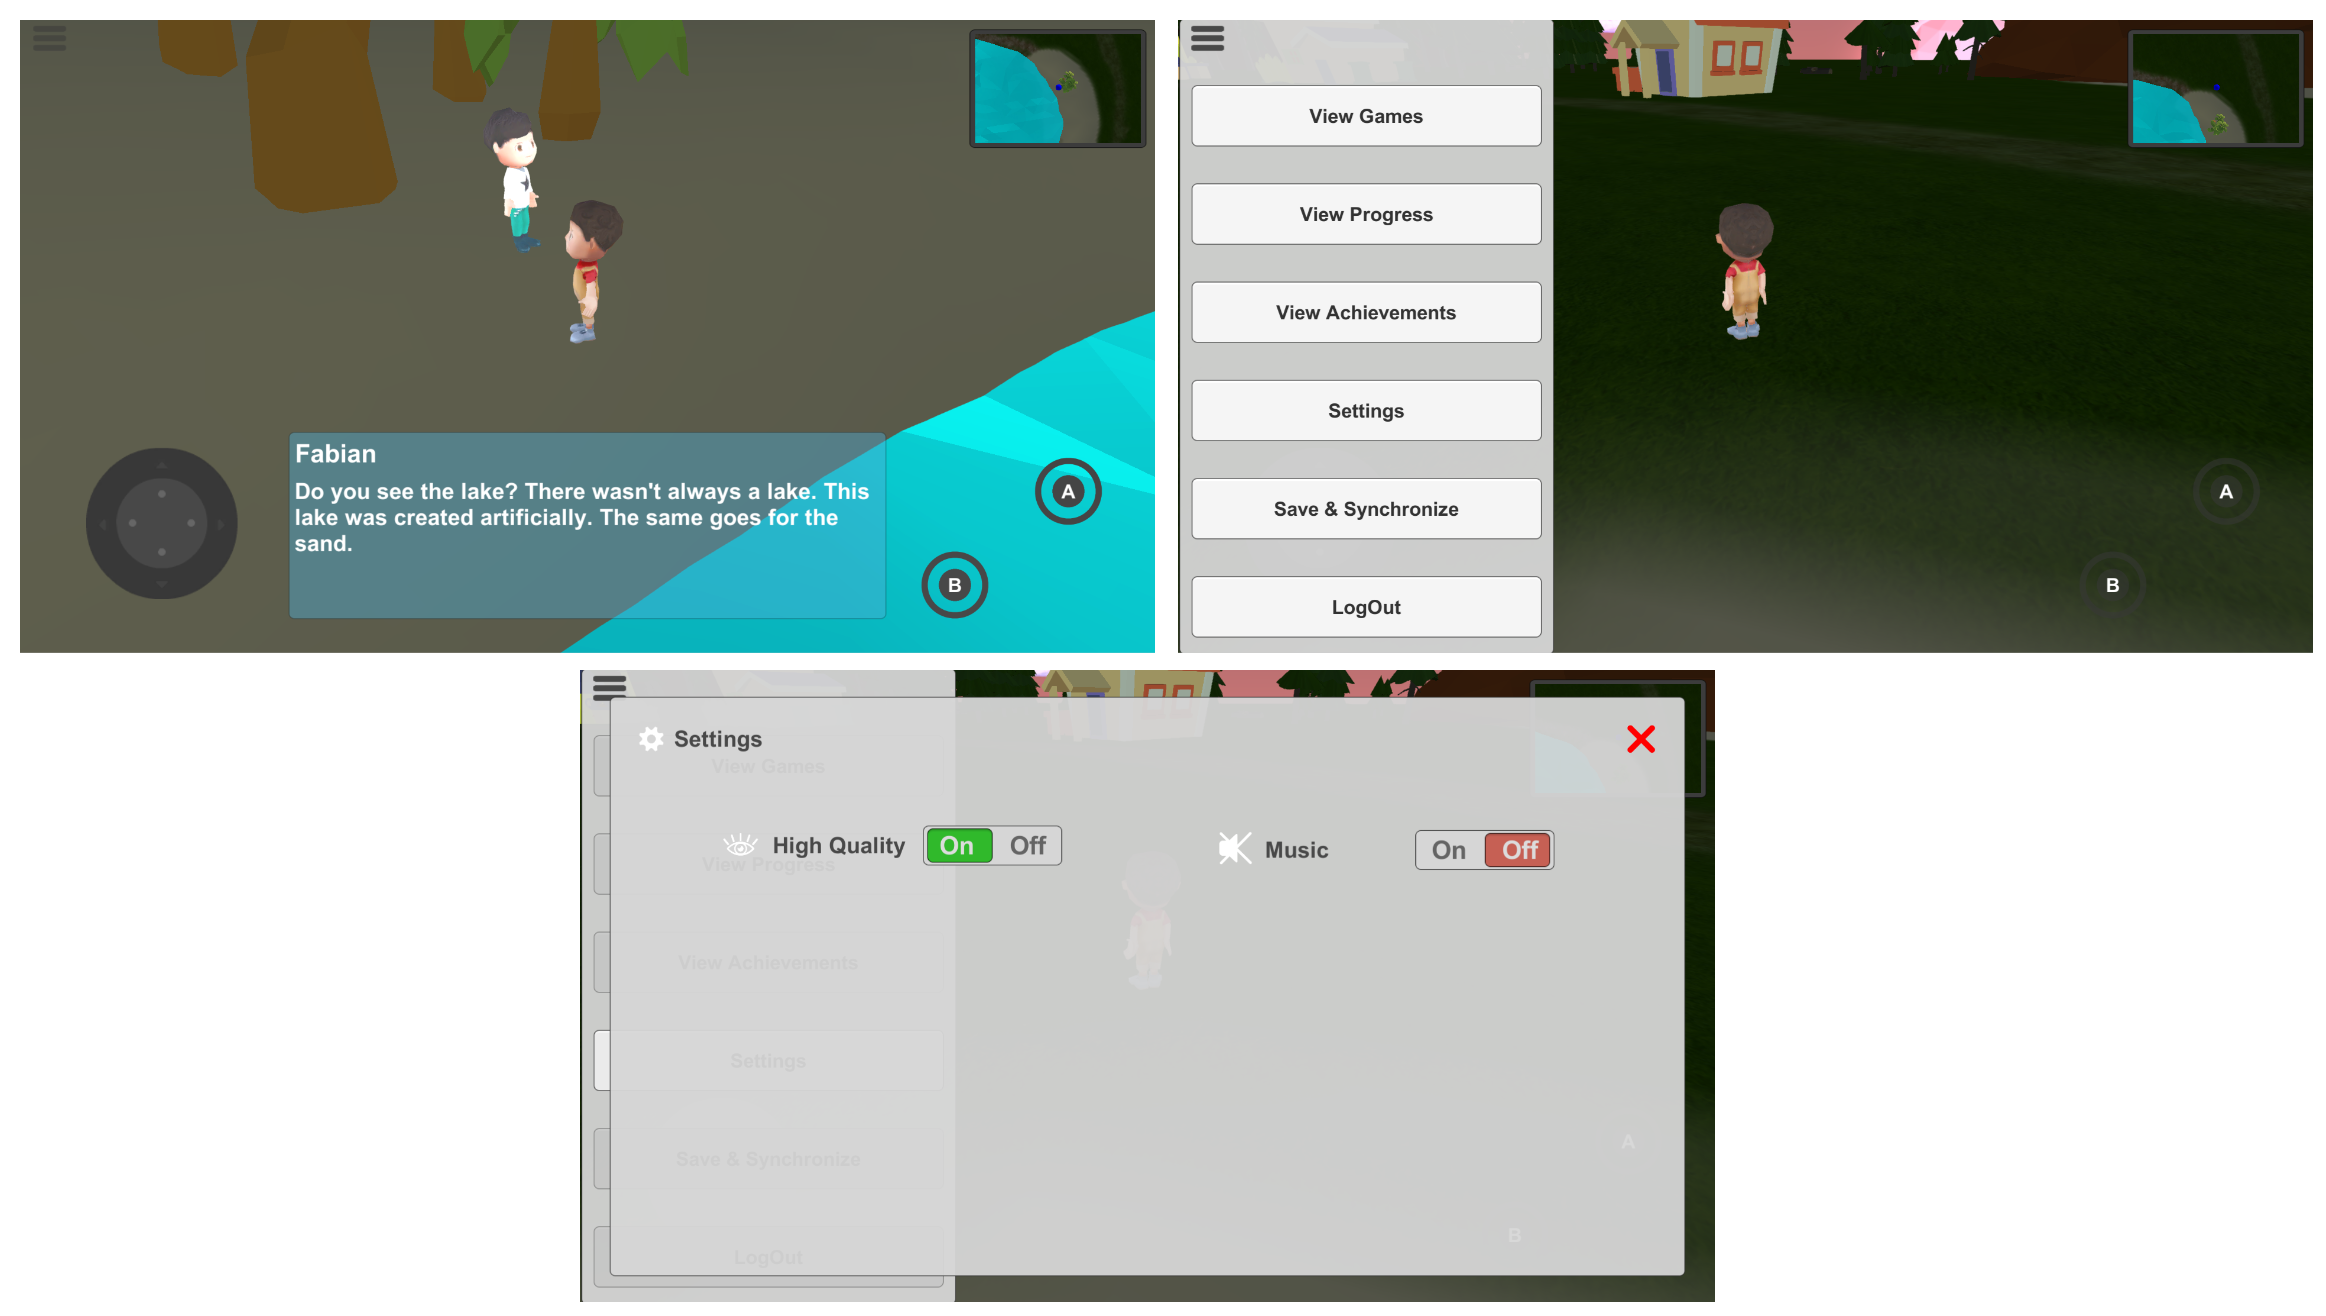
\includegraphics[width=\textwidth]{pics/userInterface.png}
			\caption{User Interfaces: Kommunikation, Menu und Einstellungen-Fenster}
		\end{figure}
	
		Menu fenster bildet die erste Dialogebene nach der Startebene. Nach diesem gibt es noch eine weitere Ebene. dieser Dialog dient zum Abbrechen, warnt vor bevorstehenden Aktionen. Die maximale Dialogebene ist also 2. 

		\begin{figure}[htbp]
			\centering 
			\label{RegisterUI}
			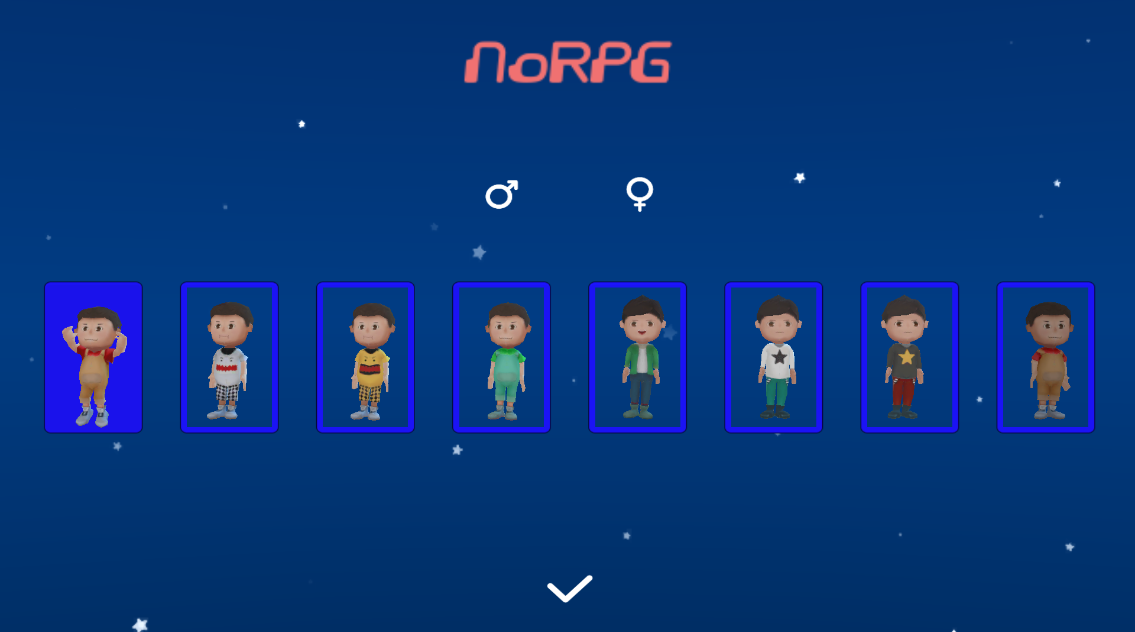
\includegraphics[width=13cm]{pics/RegisterUI.png}
			\caption{User Interface: Registrierung}
		\end{figure}

	
	\subsection{Usability Test}
		Usability TEst faken? Kinder + Jugendliche --> Katalog mit Bewertung
		Summativer TEst: Nach der Entwicklung, fertiges Produkt vor Auslieferung umfangreiche Studie
	
		Benutzerprofiele, Szenarien, Umfang, Zeitraum (3 Tage) 
	
		TEstutensilien: Prerelease version der APp und eigene Software
		Testart: Remotetest (vor und nachteile zu anderen)